\chapter{Gravitational wave detectors}\label{ch:detectors}

Detection of gravitational waves requires measuring the transverse stretching and compressing of space. The earliest attempt at this was done through resonant mass detectors, solid, vibrationally isolated cylinders tuned to a particular frequency that could be used to detect the effect of gravitational waves on the length of the cylinders~\citep{Weber_1968}. These proved incapable of reaching the required sensitivity for detecting even the strongest gravitational waves in the frequency band they were designed for ($\sim1$ kHz).

The current era of \ac{GW} detection is dominated by laser interferometers inspired by the simple Michelson interferometer. There are currently three observatories in operation: \ac{LIGO}, consisting of \ac{LHO} in Washington and \ac{LLO} in Louisiana, and the Virgo observatory in Italy. Additional detectors in Japan (Kagra) and India (\ac{LIGO} India) are under construction, and projects for next-generation detectors (Einstein Telescope, Cosmic Explorer, and \ac{LISA}) are on the horizon.


\section{GW interferometry}


To understand how an interferometer detects gravitational waves, consider a simple Michelson interferometer with arm lengths $L_x$ and $L_y$.
The interferometer measures the difference in the changes of its arm lengths, $\Delta L = \Delta L_x - \Delta L_y$, by splitting a laser beam down each arm via a beam splitter placed at the vertex, having the light reflected back by a mirror (called a \textit{test mass}) at the end of each arm, and producing an interference pattern when the beams reunite.
Differential changes in arm length manifest as phase shifts in the output.
In a LIGO detector, a photodetector is placed at the anti-symmetric output port (the output not leading back to the laser source).
The detector is tuned (by the choice of arm length) to operate at its dark fringe, i.e. the photodetector observes no signal due to destructive interference.
If one interferometer arm is elongated relative to the other, the phase shift between the signals from both arms results in some constructive interference; thus the amplitude of a gravitational wave passing through the plane of the detector arms is converted to an amplitude in laser light measured at the output port.

A gravitational wave passing through the instrument induces a \textit{strain} $h = \Delta L / L$.
Our ability to measure gravitational waves therefore depends on how precisely we can measure $\Delta L$ and how long we construct the interferometer arms to be.
The photodiode is ultimately limited by \textit{shot noise}, the random fluctuations in the number of photons observed.
This is a Poisson process, so the fluctuations scale with the square root of the photon count $N_{\mathrm{photon}}$, which itself is dependent on the laser power and wavelength and the frequency of the GW signal we are searching for:
\begin{equation}
  N_{\mathrm{photon}} \sim \frac{P_{\mathrm{laser}} \lambda_{\mathrm{laser}}}{h c f_{\mathrm{GW}}}.
\end{equation}
The minimum detectable differential arm length change for a photodiode limited by shot noise is
\begin{equation}
  \Delta L \sim \frac{N_{\mathrm{photon}}^{1/2}}{N_{\mathrm{photon}}} \lambda_{\mathrm{laser}}
\end{equation}
which gives a minimum detectable strain, for a kilometer-scale interferometer with a 1-$\mathrm{\mu}$m, 1-W laser observing 300-Hz gravitational waves is $h \sim 10^{-17}$.
This is impressive but still a ways from being able to observe the GW sources discussed in the previous chapter ($h \lesssim 10^{-20}$).

We can also extend the interferometer, but to get an order of magnitude improvement requires an order of magnitude extension of the arms, which is not entirely practical.
Instead, we can increase the \textit{effective arm length} by designing the arms as Fabry-P\'erot cavities, forcing the light in the arms to bounce back and forth many times before returning to the beam splitter.
This works as long as the light does not spend an amount of time comparable to the passing of a full gravitational wave, so the effective arm length should not exceed $L_{\mathrm{eff}} \sim \lambda_{\mathrm{GW}}$.
For signals in the hundreds of Hertz, this limits the effective arm length to a few hundred kilometers, or a few hundred round trips for a LIGO detector.
Nevertheless, combined with the optimal photodiode above, this setup can detect a strain of $h \sim 10^{-20}$.


\section{Advanced LIGO}

The LIGO detectors completed the transition to their current design stage, \ac{aLIGO}, in 2015, and began began first observing run (\acs{O1}) on September 12 that year, making the first detection of a \ac{GW} from a \ac{BBH} merger on September 14~\citep{gw150914}.
This was followed by two more \ac{BBH} detections before the end of the run on January 16, 2016~\citep{gwtc1}.
\Ac{O2} started on November 30, 2016 after a period of detector upgrades and ended on August 25, 2017.
During that run, in addition to several more \ac{BBH} detections, the \ac{LIGO} network (with the addition of the Virgo detector in Italy towards the end of the run) observed the first \ac{BNS} merger on August 17, 2017~\citep{gw170817}.
\Ac{O3}, which spanned April 1, 2019 to March 27, 2020, came after another round of major improvements in the performance of the detectors~\citep{Buikema_2020} and the full inclusion of the Virgo detector in the \ac{GW} network.
By the end of O3, the LIGO and Virgo detectors had observed an all-time total of 90 GW events~\citep{gwtc2,gwtc3}.

The performance of the LIGO detectors can be assessed in terms of its astrophysical range and its duty cycle.
The range is the distance at which a detector can observe a given GW source; in O3, LHO and LLO had binary neutron star inspiral ranges of about 111\,Mpc and 134\,Mpc, respectively.
Their duty cycles, the percentage of time each was in science observation mode, were 75\% and 77\%, with a joint-observing duty cycle of 62\%.

A number of technological advances building on top of the basic Fabry-P\'erot interferometer design have allowed the current generation of detectors to achieve their incredible sensitivity~\citep{aLIGO_design}.
Increasing laser power and injecting squeezed light reduces the effects of shot noise.
A power recycling cavity at the symmetric output sends the constructively-interfering light leaving in that direction back into the interferometer (essentially increasing laser power).
A signal recycling cavity at the anti-symmetric output is used to modify the shape the of detector response function, effectively tuning it to be more sensitive to a specific frequency band.

We now walk through the full journey on which the interferometer laser embarks, giving names to the various components of the aLIGO detector as these will be relevant in later discussions of detector noise and instrumentation.
The laser is produced at the start of the \textit{input arm}.
In O3, this \ac{PSL} is amplified to 70\,W before entering the main beam tube of the interferometer, where it then passes through an \ac{IMC} optical cavity that filters out higher-order spatial beam modes.
The \ac{IMC} optics are located inside two vacuum chambers called \acp{HAM} (namely HAM2 and HAM3) spanning the mode cleaner tube, which comprises the majority of the input arm length.
As it reaches the interferometer vertex, the beam is split into two by the beam splitter.
In each arm, it passes through an \ac{ITM}, beyond which it has entered a 4-km-long Fabry-P\'erot cavity.
The beams now leave the \textit{corner station} en route to the \textit{end stations} (End-X and End-Y) where the \acp{ETM} are housed.
Between the \acp{ITM} and \acp{ETM} the laser bounces some 300 times before returning to the beam splitter.
The carrier light exits along the input arm and enters the power recycling cavity, whose optics are located in the same \ac{HAM} chambers as the \ac{IMC} optics.
In the \textit{output arm}, the signal recycling cavity (in HAM4 and HAM5) extracts the GW signal from the exiting signal sidebands, transmitting them to the \ac{OMC} (in HAM6) which again filters out higher-order modes.
This is also where squeezed vacuum state is injected into the interferometer to reduce shot noise.
Finally, the output photodiode in HAM6 receives the signal light, which is converted by the calibration system into a gravitational wave strain measurement.


\section{Noise sources}

We have seen that photon shot noise limits the sensitivity of any GW interferometer, and is reduced by using a high-power input laser.
However, increasing laser power brings up a second noise source, similarly associated with the quantum mechanical behavior of light.
The force of the laser light hitting the test masses causes fluctuations in the test mass positions, referred to as \textit{radiation pressure noise}.
These random displacements similarly limit the sensitivity, although in contrast with shot noise they fall off with the GW frequency.
Radiation pressure is addressed by increasing the size of the test masses themselves (40\,kg in the aLIGO detectors).

\begin{figure}
  \centering
  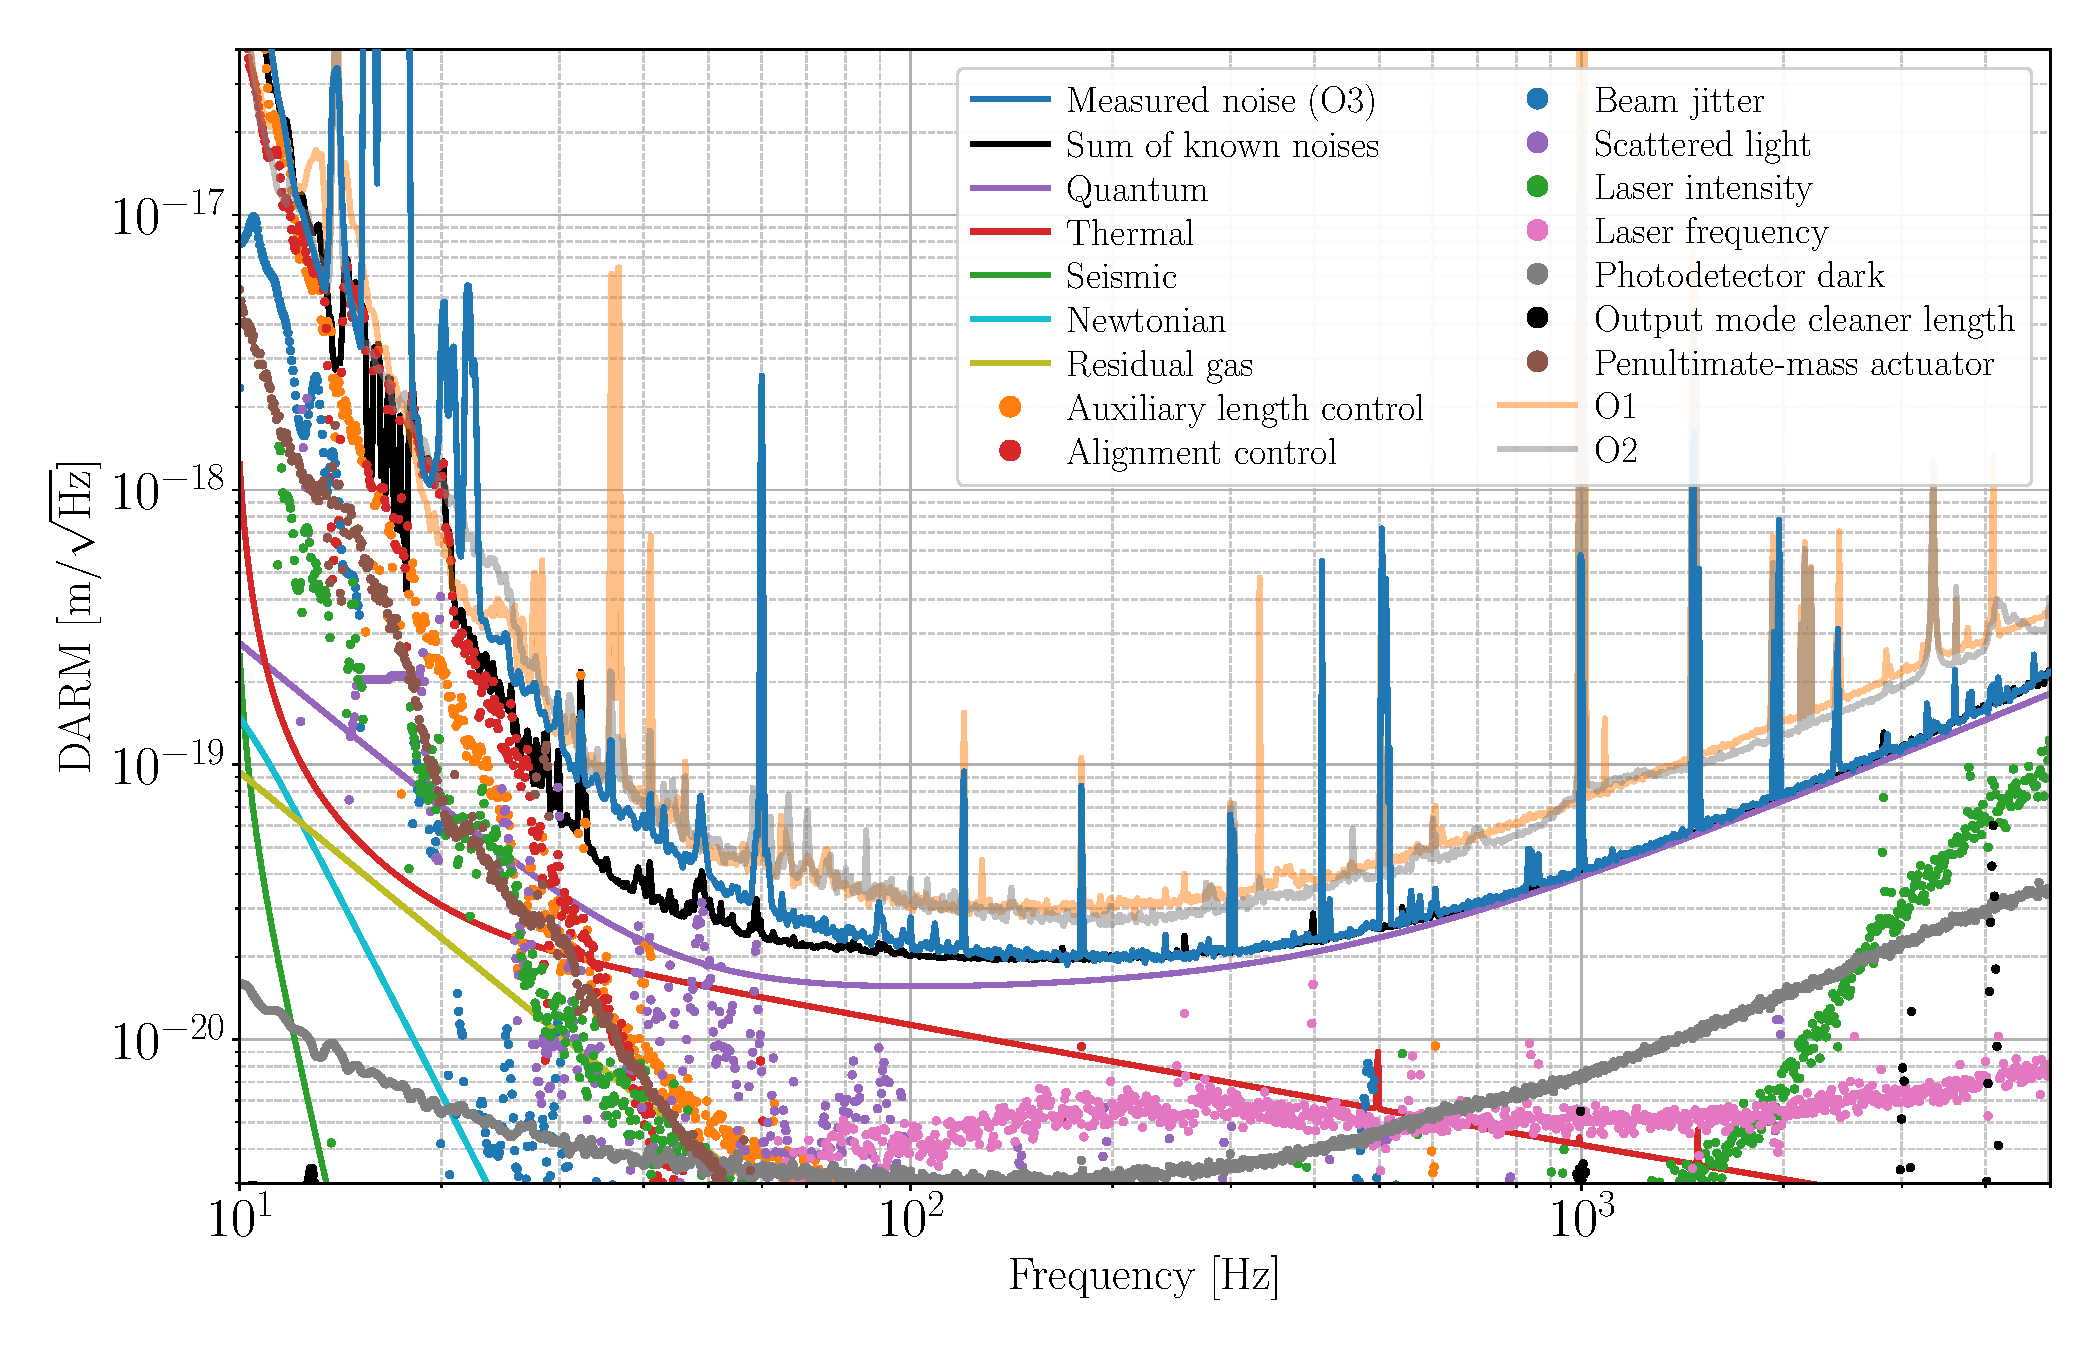
\includegraphics[width=\textwidth]{figures/detectors/budget-lho.pdf}
  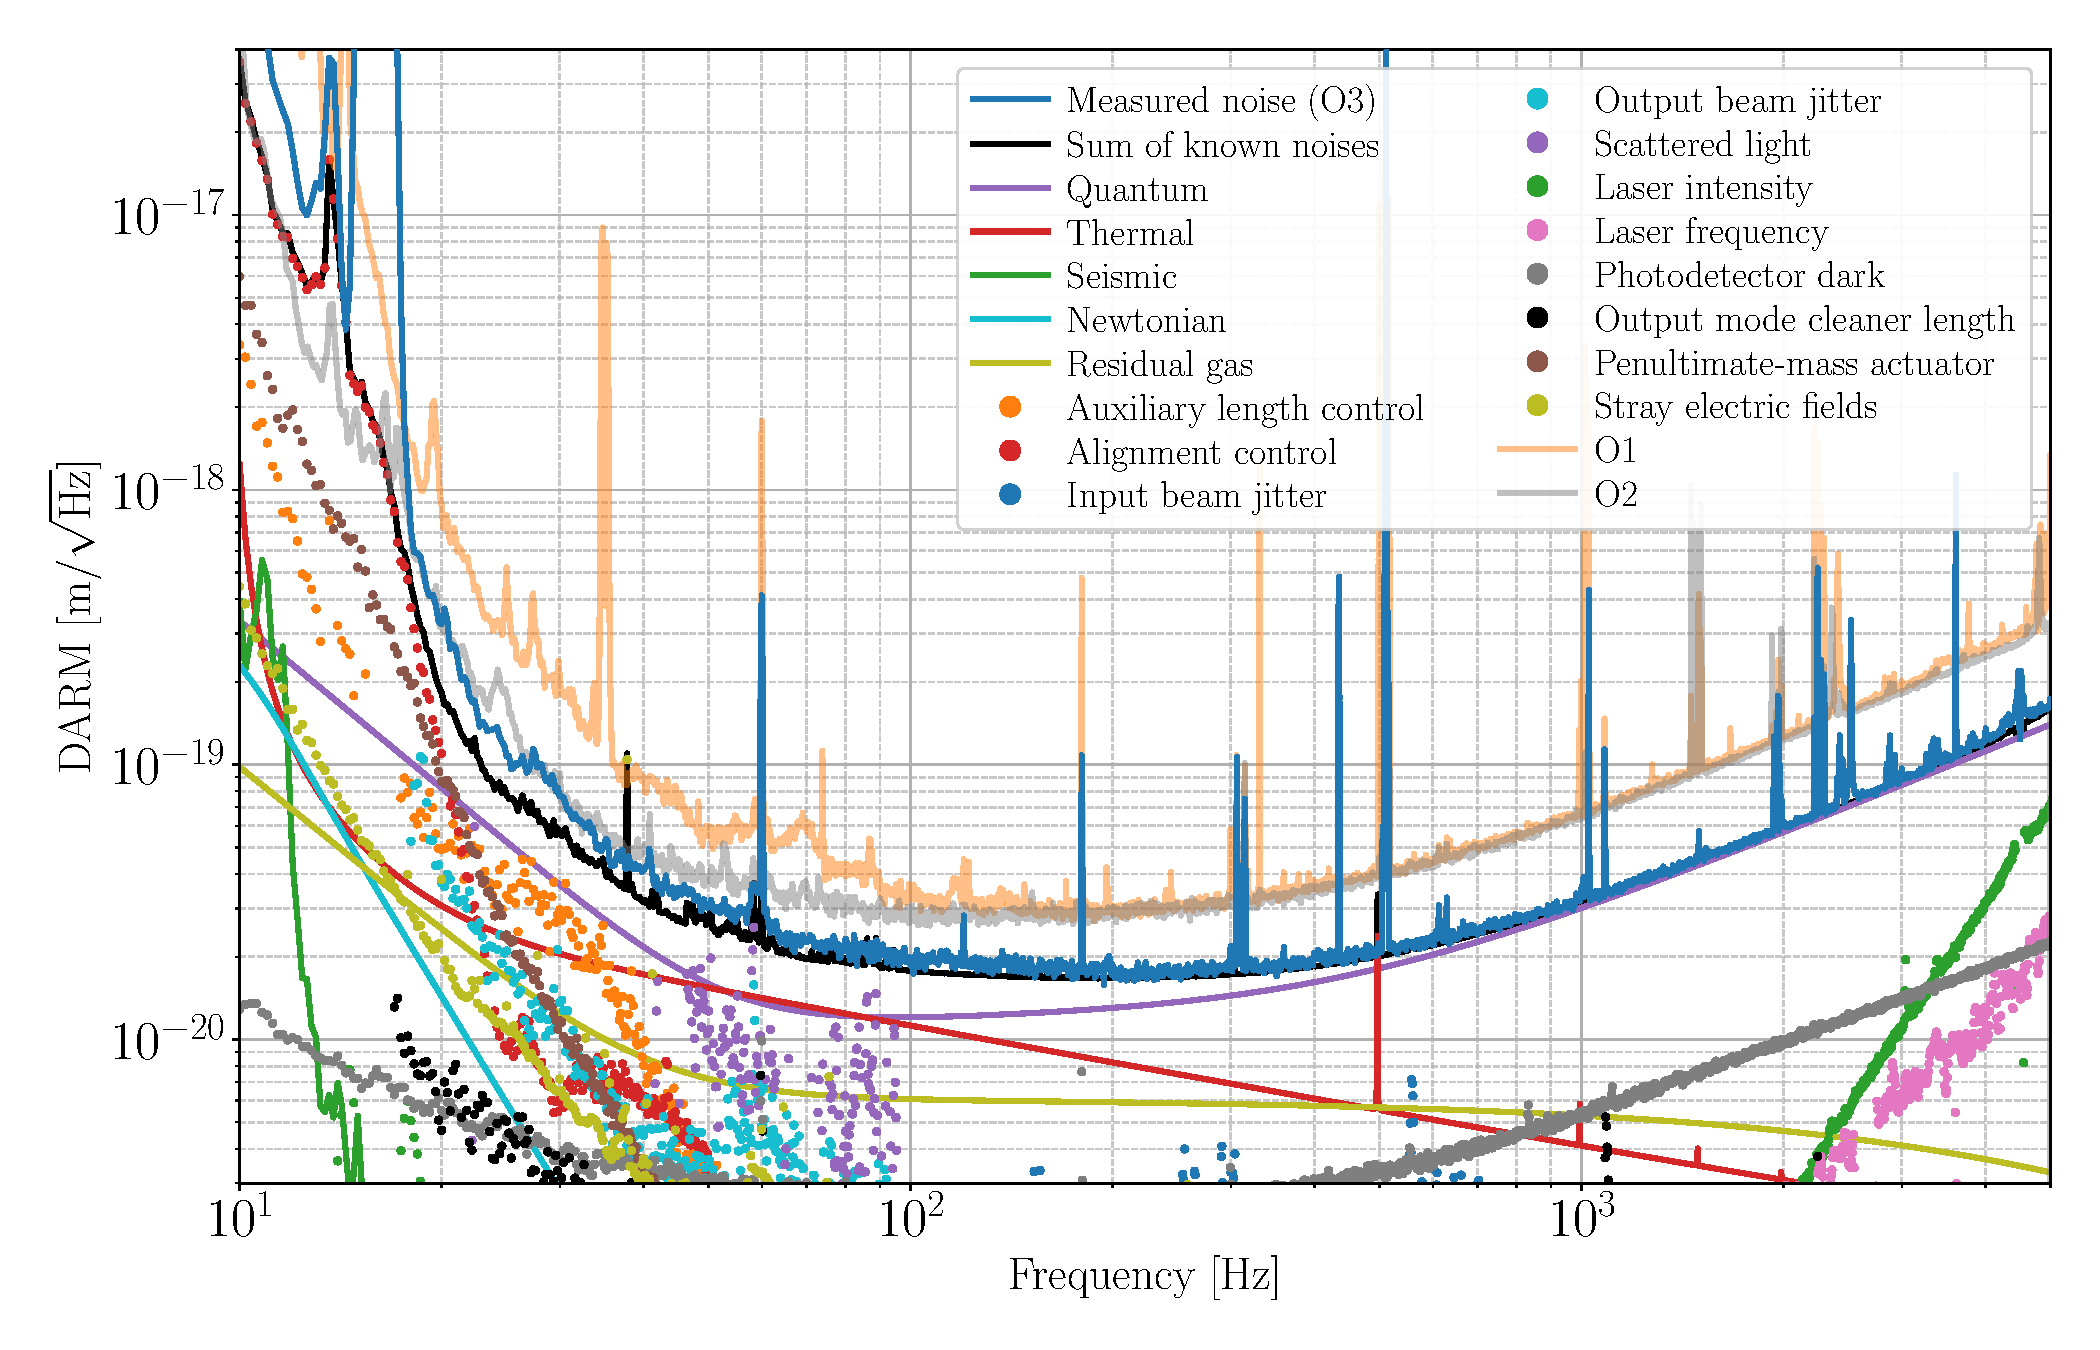
\includegraphics[width=\textwidth]{figures/detectors/budget-llo.pdf}
  \caption
  [Full noise budgets of the LIGO Hanford (top) and Livingston (bottom) observatories at the end of the third observing run.]
  {Full noise budgets of the LIGO Hanford (top) and Livingston (bottom) observatories at the end of the third observing run. ``Quantum'' noise refers to both shot noise and radiation pressure noise. Reproduced from~\protect\citet{Buikema_2020}.}
  \label{fig:detectors-budget}
\end{figure}

In addition to the quantum mechanical limitations of shot noise and radiation pressure noise, there are a plethora of noise sources not intrinsic to the design of an interferometer.
Figure~\ref{fig:detectors-budget} shows measurements and estimates of all known noise sources affecting both LIGO detectors at the end of \ac{O3}.

At low frequencies there is \textit{seismic noise}, which comes from ground motion caused by seismic and human activity.
The core optics must be suspended on multi-stage isolation systems to dampen these movements; otherwise they would completely swamp out the tiny fluctuations induced by gravitational waves.
The transfer function of a pendulum, derived by taking the Fourier transform of the simple pendulum equation of motion, describes the attenuation of motion it provides:
\begin{equation}
  A(f) = \frac{1}{1 - (f / f_{\mathrm{pend}})^2}
\end{equation}
where $f_{\mathrm{pend}} \equiv \sqrt{g/l} / (2\pi)$ is its natural frequency.
Designing a pendulum with low $f_{\mathrm{pend}}$, i.e. a long one, allows substantial attenuation above that frequency, but it can be physically impractical to go too long.
Rather, stacking multiple pendulums each with a low enough $f_{\mathrm{pend}} \lesssim 1\,Hz$, each providing a $\propto f^{-2}$ attenuation, results in much better damping in the tens of Hertz.
This construction suppresses the contribution of seismic noise to orders of magnitude below that of other noise sources, except at the very low frequencies $f \lesssim f_{\mathrm{pend}}$ outside of the LIGO detection band.

Brownian motion of molecules in the test masses themselves results in \textit{thermal noise}, which is dependent on the temperature of the optics.
Thermal noise excites the internal vibrational modes of the test masses, as well as the ``violin'' modes of the glass fiber suspensions that make up the final pendulum stage.
These modes have very high Q-factors, resulting in the very loud, narrow lines at their resonances ($\sim 500$\,Hz).

\textit{Scattered light noise} occurs when the laser beam reflecting off the beam spot on a test mass or other optic ends up hitting surfaces that are moving relative to the optic, like vacuum chamber walls.
A very small fraction of the light reaching the moving surface is reflected to the originating or another beam spot, where it scatters back into the main interferometer beam.
As the distance to the moving surface changes, the phase of the returning light changes relative to the main beam, producing fluctuations in the amplitude of the beam, that, at just 1 part in $10^{20}$ can be on the scale of those produced by gravitational waves.
In addition to this sensitivity to recombined scattered light, the scattering noise is problematic because of non-linear coupling when the path length modulation becomes comparable to the wavelength of the light, producing noise at harmonics of modulation frequencies~\citep{Soni_2020}.

The input laser system can itself be a source of \textit{beam jitter noise}.
Alignment fluctuations in the beam, called jitter, cause variations in the coupling of the fundamental optical mode to the arm cavities~\citep{Mueller_2005, Hardwick_2019}.
In principle the symmetry of the interferometer arms should reject the effects of jitter, but defects in the test masses can break this symmetry, resulting in significant noise at the jitter frequencies, which are typically associated with mechanical resonances of optic mounts the input laser table.

All of the above represent mechanical influences on the strain measurement.
However, even oscillating magnetic fields can affect components of the detector, causing \textit{magnetic field noise}.
The fields can couple by directly affecting permanent magnets on or near the test masses.
In Initial LIGO, permanent magnets were placed on the test mass suspensions as well as on the test masses themselves; the test mass ones were removed prior to \ac{LIGO}, so only the magnets on the suspension systems remain.
The suspension system suppresses permanent magnet displacement $\propto f^{-2}$, so it is only likely to dominate at low frequencies.
At higher frequencies, magnetic noise is dominated by the induction of currents in the various cables and connectors that are part of the interferometer control system.
These effects may be unpredictable: changes to electronic hardware are made frequently, each time potentially introducing a new source of noise or modifying an existing one.
